% !TEX TS-program = pdflatex
% !TEX encoding = UTF-8 Unicode

% This is a simple template for a LaTeX document using the "article" class.
% See "book", "report", "letter" for other types of document.

\documentclass[10pt]{article} % use larger type; default would be 10pt
\usepackage[utf8]{inputenc} % set input encoding (not needed with XeLaTeX)
\usepackage{framed}
\usepackage[utf8]{inputenc}
\usepackage[T1]{fontenc}
\usepackage{csquotes}
\usepackage{booktabs}
\usepackage{wrapfig}
\usepackage[english]{babel}
\usepackage{blindtext}
\usepackage{subcaption}
\usepackage{lettrine}
%%% Examples of Article customizations
% These packages are optional, depending whether you want the features they provide.
% See the LaTeX Companion or other references for full information.

%%% PAGE DIMENSIONS
\usepackage{geometry} % to change the page dimensions
\setlength{\abovecaptionskip}{10pt plus 5pt minus 3pt}
\usepackage{wrapfig}
\geometry{a4paper} % or letterpaper (US) or a5paper or....
% \geometry{margin=2in} % for example, change the margins to 2 inches all round
% \geometry{landscape} % set up the page for landscape
%   read geometry.pdf for detailed page layout information

\usepackage{graphicx} % support the \includegraphics command and options
\usepackage{amsthm, amsmath, wasysym, MnSymbol}
\usepackage{booktabs} % Top and bottom rules for table
\usepackage[font=small,labelfont=bf]{caption} % Required for specifying captions to tables and figures
% \usepackage[parfill]{parskip} % Activate to begin paragraphs with an empty line rather than an indent

%%% PACKAGES

\usepackage{booktabs} % for much better looking tables
\usepackage{array} % for better arrays (eg matrices) in maths
\usepackage{paralist} % very flexible & customisable lists (eg. enumerate/itemize, etc.)
\usepackage{verbatim} % adds environment for commenting out blocks of text & for better verbatim
%\usepackage{subfig} % make it possible to include more than one captioned figure/table in a single float
% These packages are all incorporated in the memoir class to one degree or another...

%%% HEADERS & FOOTERS
\usepackage{fancyhdr} % This should be set AFTER setting up the page geometry
\pagestyle{fancy} % options: empty , plain , fancy
\renewcommand{\headrulewidth}{0pt} % customise the layout...
\lhead{}\chead{}\rhead{}
\lfoot{}\cfoot{\thepage}\rfoot{}
%%% SECTION TITLE APPEARANCE
\usepackage{sectsty}
\allsectionsfont{\sffamily\mdseries\upshape} % (See the fntguide.pdf for font help)
% (This matches ConTeXt defaults)

%%% ToC (table of contents) APPEARANCE
\usepackage[nottoc,notlof,notlot]{tocbibind} % Put the bibliography in the ToC
\usepackage[titles,subfigure]{tocloft} % Alter the style of the Table of Contents
\renewcommand{\cftsecfont}{\rmfamily\mdseries\upshape}
\renewcommand{\cftsecpagefont}{\rmfamily\mdseries\upshape} % No bold!

%%% END Article customizations

%%% The "real" document content comes below...
\font\loll= cmr25 at 45pt
\title{ \loll Thermal analysis on a turbulent Poiseuille flow}
\author{Felipe J. O. Ribeiro, Aristeu da Silveira Neto.}
%\date{} % Activate to display a given date or no date (if empty),
         % otherwise the current date is printed 

\begin{document}
\maketitle

\begin{figure}[h!]
	\centering
	
\includegraphics[angle=0, trim={0 1cm 0 1cm},scale=0.70]{turbulence}
	\label{turbulence}
\end{figure}

\begin{abstract}
	\noindent Fluid dynamics is a subject of great academic and industrial interest. It offers many opportunities for optimization in a variety of practical engineering problems. The modeling of thermal properties of turbulent flows is something of remarkable complexity, that can be explained mathematically by the chaotic nature of this non-linear differential analysis, fact beautifully stated in the Strogatz`s book "Nonlinear Dynamics and Chaos". The immediate result of such fact is the impossibility of an exact mathematical answer for, near, all real applications. The only way of gathering results, then, is by numerical approach, with the discretization of space and time, for an approximate result. The problem is that, in most cases, these are a so big computational problem that become inviable as the mathematical differential methodology require a big number of computers for a big amount of time. With that in mind, the present paper aims to develop a semi-exact meta-modeled approach on a turbulent Poiseuille flow thermal analysis over a channel, aiming on efficiency and accuracy when compared to the DNS solution, the most respected but computational expensive method there is. 
\end{abstract}




\pagebreak

\begin{LARGE}
	Nomenclature: 
\end{LARGE} 


	Pr = Molecular Prandtl number
	
	
	
	
	$Re$ = Reynolds number, $Re = \frac{2R \overline{U}}{\nu}$
	
	
	$Re_\tau$ = Turbulent Reynolds number, $Re_\tau = \frac{R U_\tau}{\nu}$
	
	
	
	T = temperature
	
	
	
	$T_\tau$ = Wall coordinate temperature, $\frac{q_w}{\rho c_p u_\tau}$ 
	
	
	
	
	$T_m$ = Bulk temperature 
	
	
	
	
	${U}_c$ = Velocity on channels center
	
	
	
	u , v , w = velocities components on each axis
	
	
	$u^\prime $ , $ v^\prime $ , $ w^\prime $ = Fluctuations of velocity on each axis
	
	
	$U_\tau$ = Friction velocity
	
	
	x , y , z = Cartesian classic coordinates
	
	
	$\tilde{y} $= $ y \frac{u_\tau}{R} $
	
	
	R = half of the channel length
	
	
	
	b = channel depth
	
	
	
	$\nu$ = kinetic viscosity
	
	
	$\nu_\tau$ = Turbulent viscosity
	
	
	$\rho$ = Specific mass
	
	
	$\alpha$ = Thermal diffusivity
	
	
	$\alpha_t$ = Turbulent thermal diffusivity 
	
	
	$\tilde{()}$ = Normalized under wall properties
	
	$\overline{()}$ = mean value  



\tableofcontents

\section{Introduction}

\lettrine[nindent=0em,lines=2]{I}s well known that the field of turbulent diffusion is of such hight complexity that, even nowadays, it is not completely understood, as described by O. Basim and Hasan, 2007 \cite{hasan}. Out of the domain of Direct Numerical Solutions (DNS), all sorts of experimental approximations have to be assumed to properly mathematically develop the Navier-Stokes equations as the nonlinear behavior of these systems \cite{John} make difficult for an exact mathematical solution. 

Despite the difficulty, a big part of the scientific community is studying turbulence on fluid and thermal dynamics, because of the great industrial and academic interest, as the problem offers great opportunities in optimization of machinery. In other hand, it is an example of chaotic nonlinear dynamic system, what grows in the eyes of academia.   

In this work, the mixing length model was used, by Ludwig Prandtl, that rely on the Boussinesq hypothesis for being a way of modeling the Reynolds tensor on the development of the Navier-Stokes equation.\\ 

In this context, some parameters that worth mentioning are the turbulent Prandtl number \cite{Prandtl} and the constant $A = 26$, on Cebeci`s damping formulation \cite{Cebeci}. These physical terms are responsible for modeling important properties of the fluid`s thermal diffusion and dynamics as said by S. N. Aristeu, 2018 \cite{aristeu}. Such parameters models are examples of approximations that are necessary to implement a semi analytical method, like RANS, URANS and LES \cite{aristeu}. It consists in not numerically resolving the Naiver-Stokes equation on all scales required, but instead substituting some tensors and other nonlinear therms by conceptual and experimental approximations.

Such methods are important because they offer a much quicker solution. The DNS approach demands high computational work, not even being possible or viable in some cases, as explained on H. Kawamura, H. Abe and Yuichi Matsuo's work \cite{Abe}. An example of this is for high Reynolds number systems. But, in other hand, these approximated methods result in some errors in comparison with the DNS solution.    

On the present paper, the authors aim to develop a semi analytical RANS (Reynold`s Averaged Navier-Stokes) method to describe the thermal configuration on a turbulent plane Poiseuille flow \cite{Poiseuille}, modeled with the mixture length methodology. Meta-models were developed defining the turbulent Prandtl number \cite{Prandtl} and the constant $A = 26$, on Cebeci`s damping formulation, to enhance the results compared to DNS solutions, resulting on accuracy and efficiency, what gave birth to new models for the parameters modeled. The results of this work's formulation were compared with the DNS result (\cite{DNS1020} , \cite{DNS150}), aiming to provide an analysis on the viability of meta models on turbulent Poiseuille flows thermal problems. \\       
 

\section{Physical model}

The problem was defined as a plane channel flow, with only one finite dimension on the $y$ axis. Two boundary walls were set as two nonslip infinite plates in a constant thermal flux regime. The $z$ axis was proposed self similar both on velocity and temperature, resulting on a plane domain (Fig.\ref{figure.1}). \\
The fluid was incompressible and Newtonian. It was flowing on the $x$ axis direction on Reynolds numbers that variated from $4560$ to $41441$, resulting on a turbulent regime domain. 

\begin{figure}[h!]
	\centering
	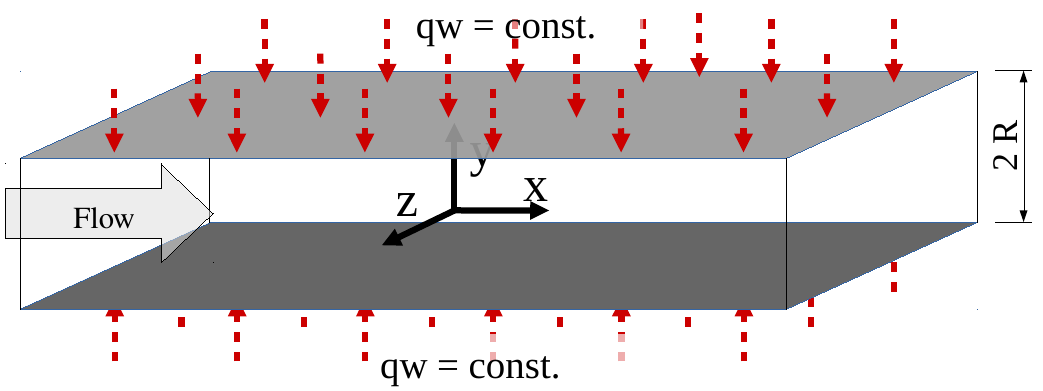
\includegraphics[angle=0, scale=0.50]{figure1}
	\caption{Geometric definition and boundary condition of the system.}
	\label{figure.1}
\end{figure}

The base mathematical formulation for the problem where the continuity and Navier-Stokes equations as defined on Cengel's book \cite{Cengel}, and the  energy transport equation, as defined on Freank's Incropera \cite{Incropera}. These were the assumptions made to the proposed problem, that will be considered on the mathematical model ahead.









\section{Differential model}

Developing the thermal energy equation, the continuity equation and the Navier-Stokes equations for mean statistical permanent regimes resulted on: 


\begin{equation}\label{energy permanent}
\frac{\partial{}}{\partial{x}} \left(\overline{T^\prime u^\prime}\right) + \frac{\partial{}}{\partial{x}}\left(\overline{u}.\overline{T}\right)     + 
\frac{\partial{}}{\partial{y}} \left(\overline{T^\prime v^\prime}\right) + \frac{\partial{}}{\partial{y}}\left(\overline{v}.\overline{T}\right) 
=
{\frac{\partial{}}{\partial{x}}} \left(\alpha {\frac{\partial{\overline{T}}}{\partial{x}}} \right) +
{\frac{\partial{}}{\partial{y}}} \left(\alpha {\frac{\partial{\overline{T}}}{\partial{y}}} \right). 
\end{equation}

\begin{equation}\label{mass}
\frac{\partial \overline{u}}{\partial x} = 0.
\end{equation}

\begin{equation}\label{dynamics}
\frac{\partial \overline{u}\overline{v}}{\partial y} = 
- \frac{1}{\rho} \frac{\partial \overline{p}}{\partial x} + \frac{\partial}{\partial y}\left(\nu \frac{\partial \overline{u}}{\partial y} - \overline{u^\prime v^\prime}\right).
\end{equation}

Where (\ref{energy permanent}) represents the mean energy balance for a given point, the (\ref{mass}) represents the mean mass balance and (\ref{dynamics}) represents de mean linaer momentum balance. What configure the method as a Reynolds Averaged Navier Stokes(RANS) methodology.

\subsection{The temperature permanent regime}

Even when on simplified mean values, the temperature field of a turbulent channel flow don't converge naturally to a unidimensional permanent state (fig.\ref{figure.2}). In a effort to simplify the solution, the thermal configuration was studied with a thermal flux equation (\ref{c_h_e}).
\begin{figure}[h!]
	\centering
	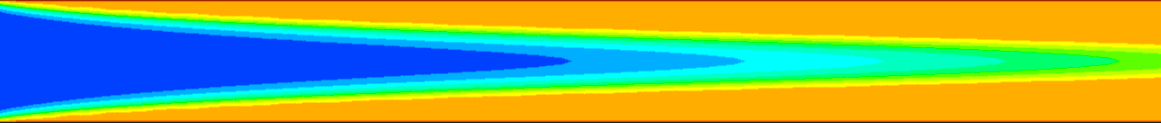
\includegraphics[angle=0, scale=0.40]{temperatura}
	\caption{Temperature field in statistical permanent regime over a channel.}
	\label{figure.2}
\end{figure}
\begin{equation}\label{c_h_e}
q_{conv.} = \dot{m} C_p \Delta T_m.
\end{equation}
\begin{equation}
2q_w b \Delta x = \dot{m} C_p \Delta T_m.
\end{equation}
Being $b$ the depth of the channel and $T_m$ the average temperature in a cross-section. So, substituting $ \dot{m} = u_m 2R b \rho $, and assuming $ \Delta T_m = \frac{\partial{\left(\overline{T}_m\right)}}{\partial{x}} \Delta x $:
\begin{equation}
2q_w b \Delta x = u_m 2R b \rho  C_p \frac{\partial{\left(\overline{T}_m\right)}}{\partial{x}} \Delta x.
\end{equation}     
\begin{equation}
q_w = u_m R \rho  C_p \frac{\partial{\left(\overline{T}_m\right)}}{\partial{x}} .
\end{equation} 
\begin{equation}\label{c_h_ee}
\frac{\partial{\left(\overline{T}_m\right)}}{\partial{x}} = \frac{q_w}{u_m  R \rho  C_p } .
\end{equation} 

As all therms on the right side are constants, the mean temperature had to varies linearly on the stream-wise direction.  
To better understand the wall temperature with such energy profile, a convective thermal flow study was made, which can be expressed mathematically by:
\begin{equation}
q_w = h A \left( T_w(x) - \overline{T}_m(x)\right).
\end{equation}
It is noted that $h$ is constant since there is a fully developed flow. Thus it is possible to write:
%\begin{equation}
%T_w(x) - \overline{T}_m(x) = \frac{q_w}{hA}.
%\end{equation}
%\begin{equation}
%\frac{d T_w(x)}{d x} - \frac{d \overline{T}_m(x)}{d x} = \frac{d \frac{q_w}{hA}}{dx}.
%\end{equation}
\begin{equation}
\frac{d T_w(x)}{d x} = \frac{d \overline{T}_m(x)}{d x} = Ctt.
\end{equation}	

With the temperature on the walls and the mean temperature gradient set as linear by these mathematical determinations, it was possible to extend this gradient to all de domain considering the boundary conditions and the symmetry of the system. So a constant temperature gradient was imposed on the heated walls, creating a boundary condition of constant thermal flux, causing all the field T(x,y) to varies linearly on the streamwise direction. The temperature value was then decomposed to the form $ T^\ast(y) = T(x,y) - T_w(x) $ where $T_w(x)$ was the temperature near the wall, resulting in a similarity effect on the streamwise direction, resuming the problem to a unidimensional representative state for the variable $T^\ast(y)$. Therefore, the expression was substituted in (\ref{energy permanent}):



\begin{equation}
\begin{split}
\frac{\partial{}}{\partial{x}} \left(\overline{(T^\ast + T_w)^\prime} \overline{ u^\prime}\right) + \frac{\partial{}}{\partial{x}}\left(\overline{(T^\ast + T_w)} \overline{u}\right)+ 
\frac{\partial{}}{\partial{y}} \left(\overline{(T^\ast + T_w)^\prime} \overline{ v^\prime}\right) + \frac{\partial{}}{\partial{y}}\left(\overline{(T^\ast + T_w)} \overline{v}\right) = \\
{\frac{\partial{}}{\partial{x}}} \left(\alpha {\frac{\partial{\overline{(T^\ast + T_w)}}}{\partial{x}}} \right) +
{\frac{\partial{}}{\partial{y}}} \left(\alpha {\frac{\partial{\overline{(T^\ast + T_w)}}}{\partial{y}}} \right) 
\end{split}
\end{equation}

Then the expression could be further developed algebraically considering all mean velocity on $y$ axis and $z$ axis null:

\begin{equation}\label{equation_var}
{\frac{\partial{}}{\partial{y}}} \left(\alpha {\frac{\partial{\overline{T^\ast}}}{\partial{y}}}   
- \left(\overline{ T^{\ast\prime} v^\prime}\right) \right)
= 
\overline{u}\frac{\partial{}}{\partial{x}}\left(\overline{T_w}\right)  
\end{equation}



\subsection{The Boussinesq hypothesis}

Now, on a unidimensional simplified expression, the model needed a closure model for the turbulent flux, for that, the Boussinesq hypothesis was used. The term $\overline{T^{\ast\prime}  v^\prime}$ 
can be developed with:
\begin{equation}\label{bou}
-\left(\overline{ u^\prime  v^\prime}\right) = 
\nu_t \frac{\partial{\overline{u}}}{\partial{y}}
\implies
-\left(\overline{ T^{\ast\prime}  v^\prime}\right) = 
\alpha_t \frac{\partial{\overline{T^\ast}}}{\partial{y}}.
\end{equation}
Thus, by substituting in the main equation (\ref{equation_var}):
\\
\begin{equation}
{\frac{\partial{}}{\partial{y}}} \left(\alpha {\frac{\partial{\overline{T^\ast}}}{\partial{y}}}   
+ \alpha_t  \frac{\partial \overline{T^\ast}}{\partial y} \right)
= 
\overline{u}\frac{\partial{}}{\partial{x}}\left(\overline{T_w}\right) . 
\end{equation}

\subsection{Prandtl mixing length model} 

Thus, arises the term of the turbulent thermal diffusion $\alpha_t$ that needs to be modeled. A new variable should be introduced, the turbulent Prandtl number, as follows:
\begin{equation}
Pr_t = \frac{\nu_t}{\alpha_t}.
\end{equation} 
So we have the $ \nu_t $ value that needed to be modeled. The value of the turbulent Prandtl number $ Pr_t = 0.71 $ that has been used in the literature.
With the model of the Prandtl mixing length, it is postulated that:
\begin{equation}
\nu_t = {l_m}^2 \left| \frac{\partial \overline{u}}{\partial y} \right|.
\end{equation}
The mixing length introduces a module into the differential model and the parameter of the turbulent Prandtl number.
\\
\begin{equation}
{\frac{\partial{}}{\partial{y}}} \left( \left( \alpha   
+ \frac{\nu_t}{Pr_t} \right) \frac{\partial \overline{T^\ast}}{\partial y} \right)
= 
\overline{u}\frac{\partial{}}{\partial{x}}\left(\overline{T_w}\right)  .
\end{equation}
\begin{equation}
{\frac{\partial{}}{\partial{y}}} \left( \left( \alpha   
+ \frac{{l_m}^2 \left| \frac{\partial \overline{u}}{\partial y} \right|}{Pr_t} \right) \frac{\partial \overline{T^\ast}}{\partial y} \right)
= 
\overline{u}\frac{\partial{}}{\partial{x}}\left(\overline{T_w}\right)  .
\end{equation}
\\

It is possible to notice, when analyzing the dynamic domain, that for positive values of $ y $ the first derivative of velocity will always be negative, since by the principles of Dirichlet and Neumman, we have a velocity that decreases with the increase of $ y $.\\
\begin{equation}
{\frac{\partial{}}{\partial{y}}} \left( \left( \alpha   
- \frac{{l_m}^2}{Pr_t}\frac{\partial \overline{u}}{\partial y} \right) \frac{\partial \overline{T^\ast}}{\partial y} \right)
= 
\overline{u}\frac{\partial{}}{\partial{x}}\left(\overline{T_w}\right)  .
\end{equation}



\subsection{The mixing length}

Then, was missing a parametrization for the mixing length $ l_m $. For this, we observed the experimental studies of Nikuradse, with which this parameter was modeled as follows.
\begin{equation}
L\left(\frac{y}{R}\right) = \frac{l_m}{R} = 0.14 - 0.08 \left(\frac{y}{R}\right)^2 - 0.06\left(\frac{y}{R}\right)^4.
\end{equation}
To further enrich the model, Cebeci and Bradshaw added the Van Driest damping function:
\begin{equation}
L\left(\frac{y}{R}\right)  = \frac{l_m}{R} = \left(\frac{l_m}{R} = 0.14 - 0.08 \left(\frac{y}{R}\right)^2 - 0.06\left(\frac{y}{R}\right)^4\right)\left\{  1 - e^{[(\tilde{y} - 1) \frac{Re_\tau}{A}]}\right\}.
\end{equation}
With $A = 26$ as the Cebeci`s constant.Thus, we had the mixing length defined by:
\begin{equation}
lm = L R.
\end{equation}
Being $ L $ a function in the $ y $ axis.
\begin{equation}
{\frac{\partial{}}{\partial{y}}} \left( \left( \alpha   
- \frac{{L}^2 R ^2}{Pr_t}\frac{\partial \overline{u}}{\partial y} \right) \frac{\partial \overline{T^\ast}}{\partial y} \right)
= 
\overline{u}\frac{\partial{}\left(\overline{T_w}\right)  }{\partial{x}}.
\end{equation}
 To compare this work with literature models more easily, the equation was nondimensionalized with the constants according to wall coordinates. It was considered: $ \tilde{y} = \frac{y . Re_\tau}{R} $, $ \tilde{\overline{u}} = \frac{\overline{u}}{u_\tau} $ , $ \tilde{\overline{T}} = \frac{\overline{T}}{T_\tau} $ , $Re_\tau = \frac{u_\tau R}{\nu}$, $Pr_t = \frac{\nu_t}{\alpha_t}$, $Pr = \frac{\nu}{\alpha}$ e $T_\tau = \frac{q_w}{\rho C_p u_\tau}$, $\frac{\partial{\left(T_m\right)}}{\partial{x}} = \frac{q_w}{u_m  R \rho  C_p } $, $\frac{\partial \overline{p}}{\partial x} = - \frac{u_\tau^2 \rho}{R} $.
\\
\begin{equation}
{\frac{\partial{}}{\partial{\tilde{y}}}} \left( \left( \frac{Re_\tau}{Pr}   
- \frac{{L}^2 Re_\tau ^3}{Pr_t}\frac{\partial \tilde{\overline{u}}}{\partial \tilde{y}} \right) \frac{\partial \tilde{\overline{T^\ast}}}{\partial \tilde{y}} \right)
= 
\frac{\tilde{\overline{u}}}{\tilde{u_m}}.
\end{equation}
It is important to note how there is velocity in the main equation, that is, for the development of the thermal domain, the development of the dynamic channel profile was necessary. For this, a previously established RANS methodology was used, as follows:
\begin{equation}
\frac{\partial \tilde{\overline{u}}}{\partial \tilde{y}} = - \frac{2 \tilde{y} \frac{1}{Re_\tau} }{ 1 + \sqrt{ 1 + 4 L ^2 Re_\tau ^2 \tilde{y}}}.
\end{equation}		
In this way, we had the first derivative of velocity in an exact form.


\section{Numerical model}


To discretize the space, an Eulerian domain was formulated. For the velocity a fourth-order Runge-kutta method was applied, while the temperature was arranged in a central differences scheme that had to be solved implicitly. The dynamic domain was solved first, and its numerical result were used in the development of the thermal profile. As for cell location, a cell center was determined on the wall, and a point between cells in the center of the channel, the rest of the space units being evenly distributed throughout the channel.
\begin{figure}[!h]
	\centering
	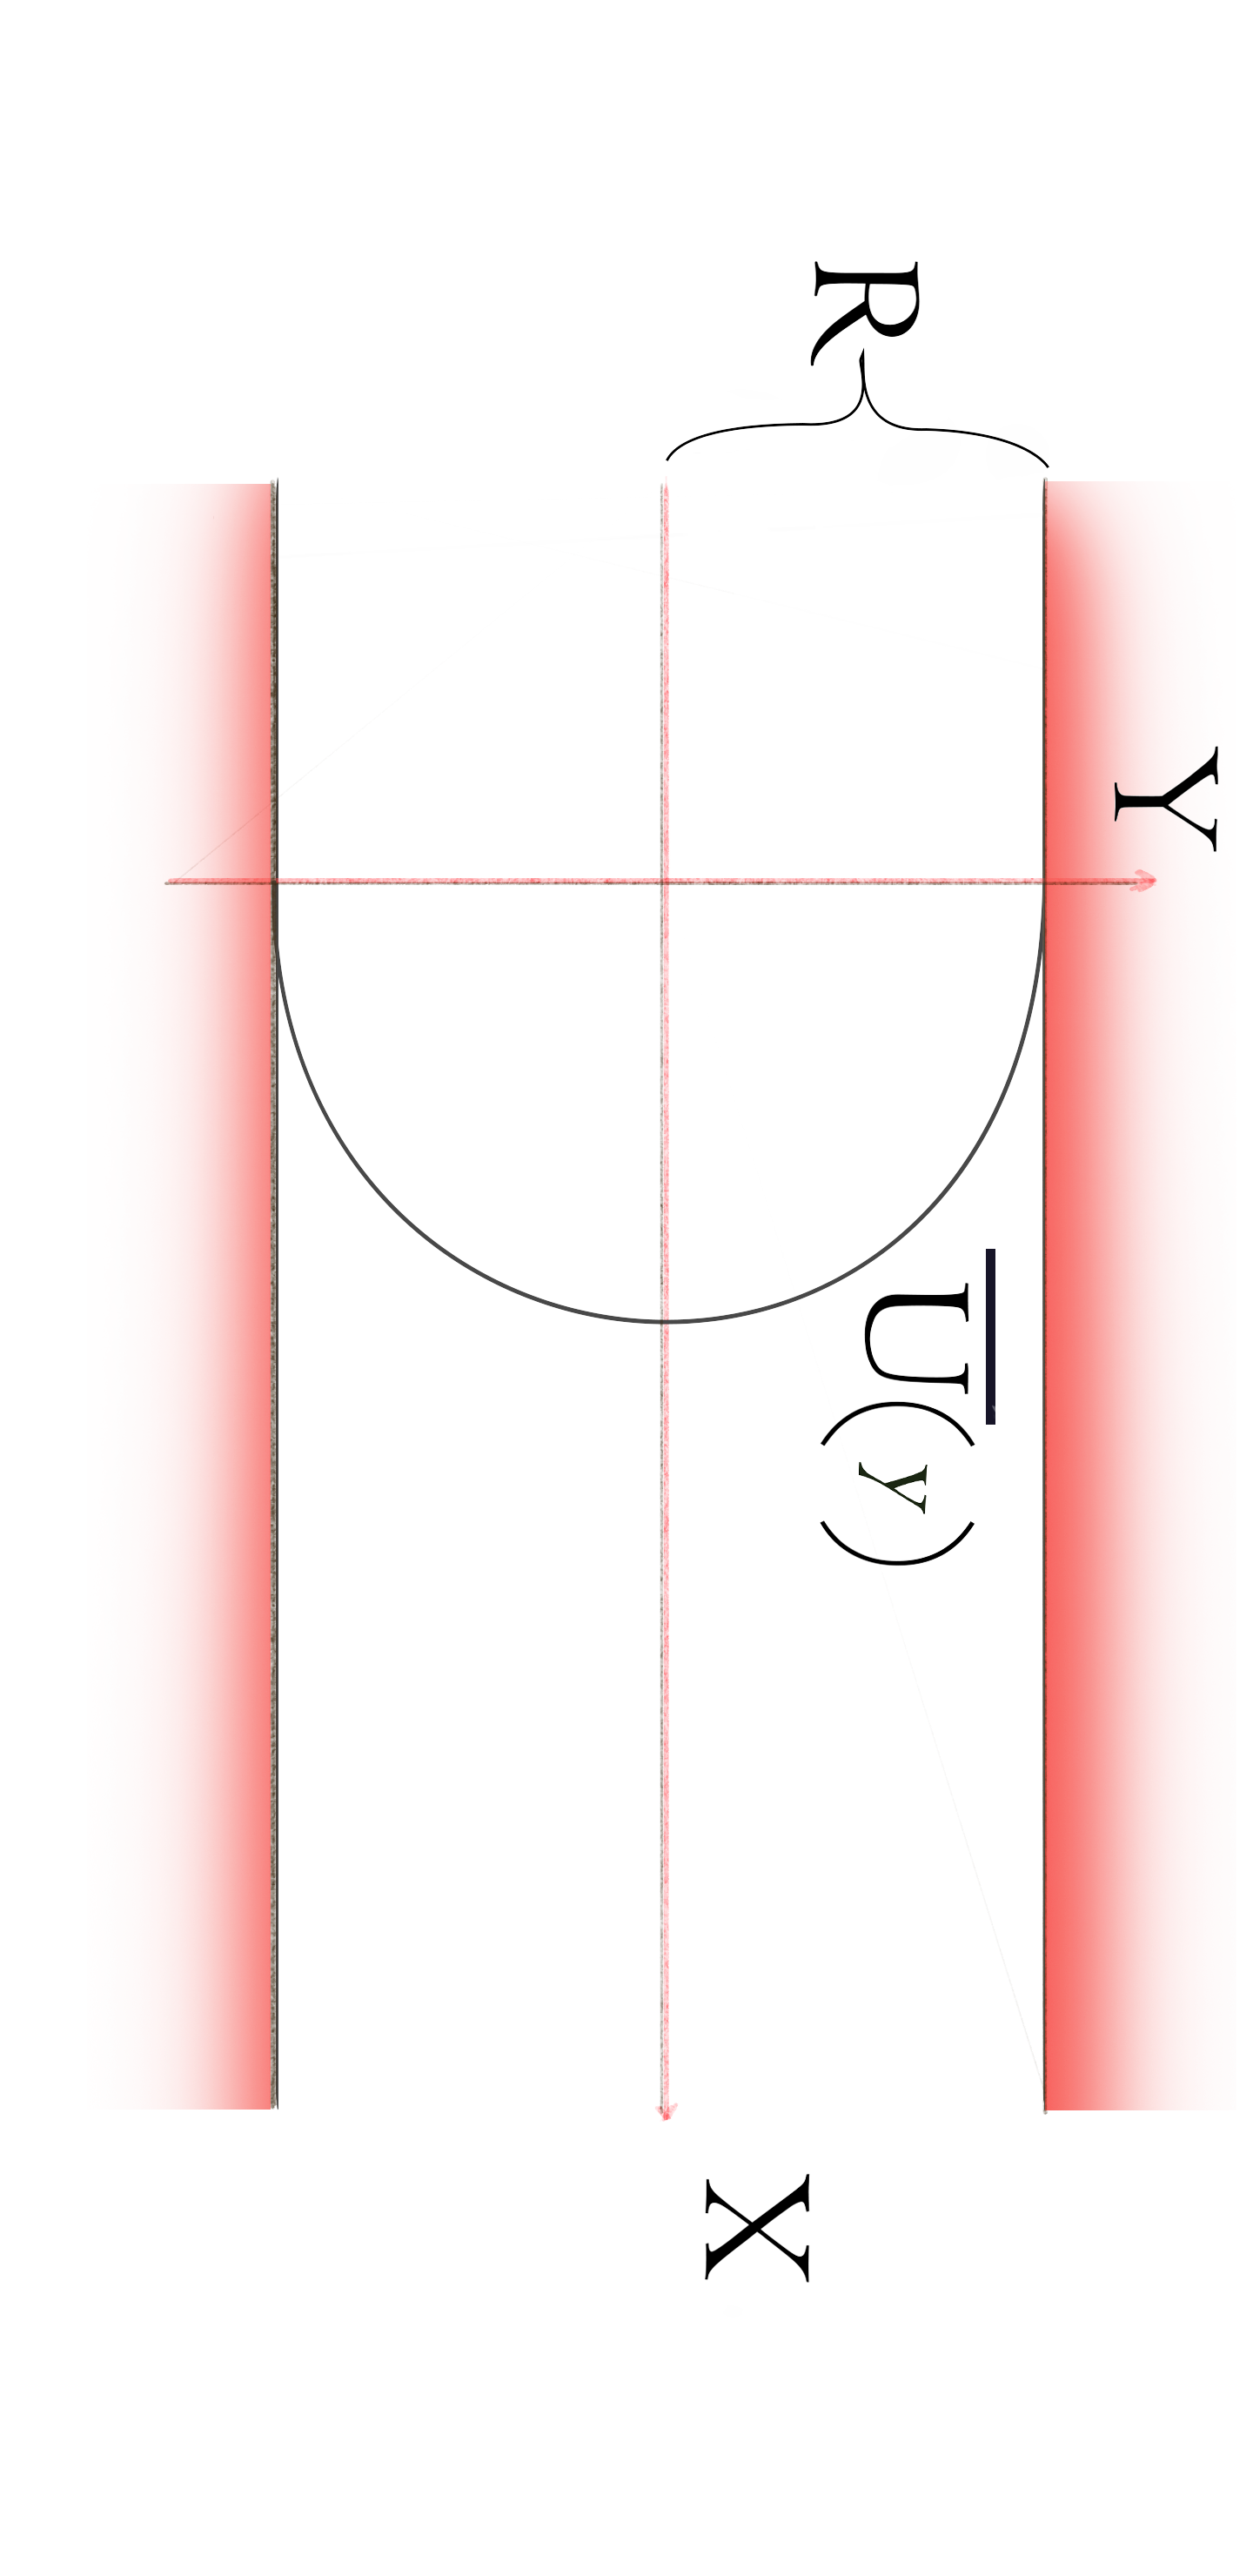
\includegraphics[angle=90, scale=0.06]{canalvermelho}
	\caption{Graphical representation of the system domain.}
	\label{sistema}
\end{figure}

\subsection{Preliminary results}
Initially the turbulent Prandtl number was used as in the literature, a value of 0.71, where the results were:\\
	\begin{figure*}[h!]
		\centering
		\begin{subfigure}[t]{0.45\textwidth}
		\centering
		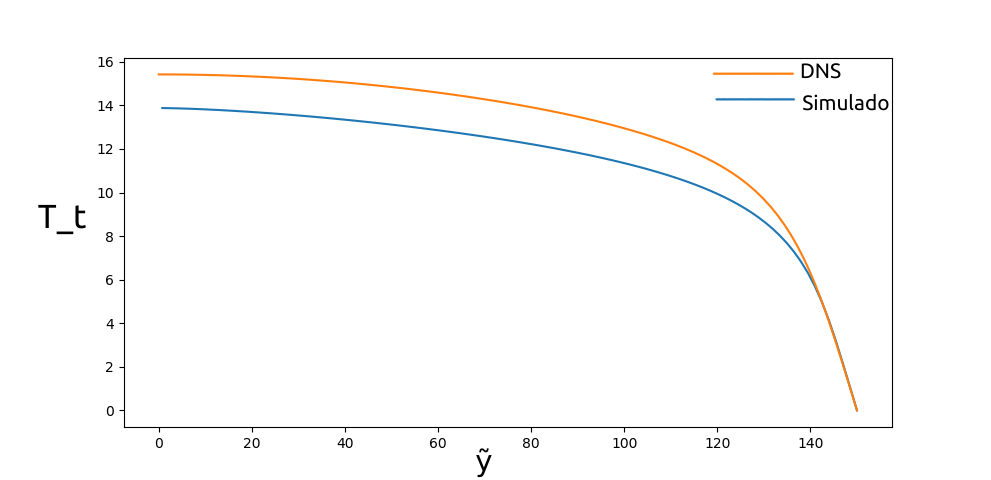
\includegraphics[angle=0, scale=0.24]{150orto}
		\caption{Results for $Re_\tau = 150$. L2 = 1.36 }
		\end{subfigure}%
		~
		\begin{subfigure}[t]{0.45\textwidth}
		\centering
		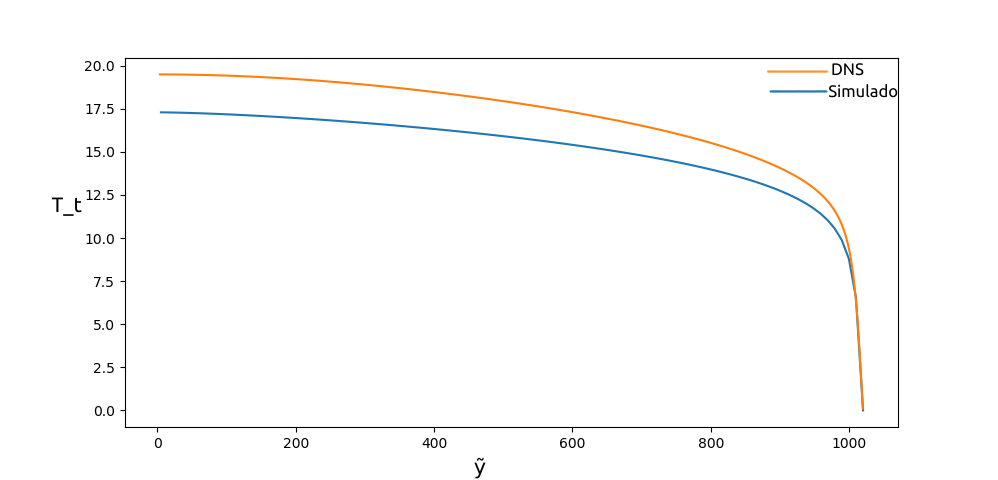
\includegraphics[angle=0, scale=0.24]{1020orto}
		\caption{Results for $Re_\tau = 1020$. L2 = 1.77}
		\end{subfigure}
	\caption{For $Pr_t = 0.71$ and $A = 26$} 
	\end{figure*}	

First results weren't satisfactory. Then, it was noticed that the turbulent Prandtl number had great influence on the outcome, so the turbulent Prandtl number from the DNS was used as a parameter in the program, obtaining an L2 norm of $ 0.19 $ to $ Re_t = 640 $. Thus it was identified that the problem was in the parametrization of the turbulent Prandtl number. It became the focus of the research.

\begin{figure*}[h!]
	\centering
	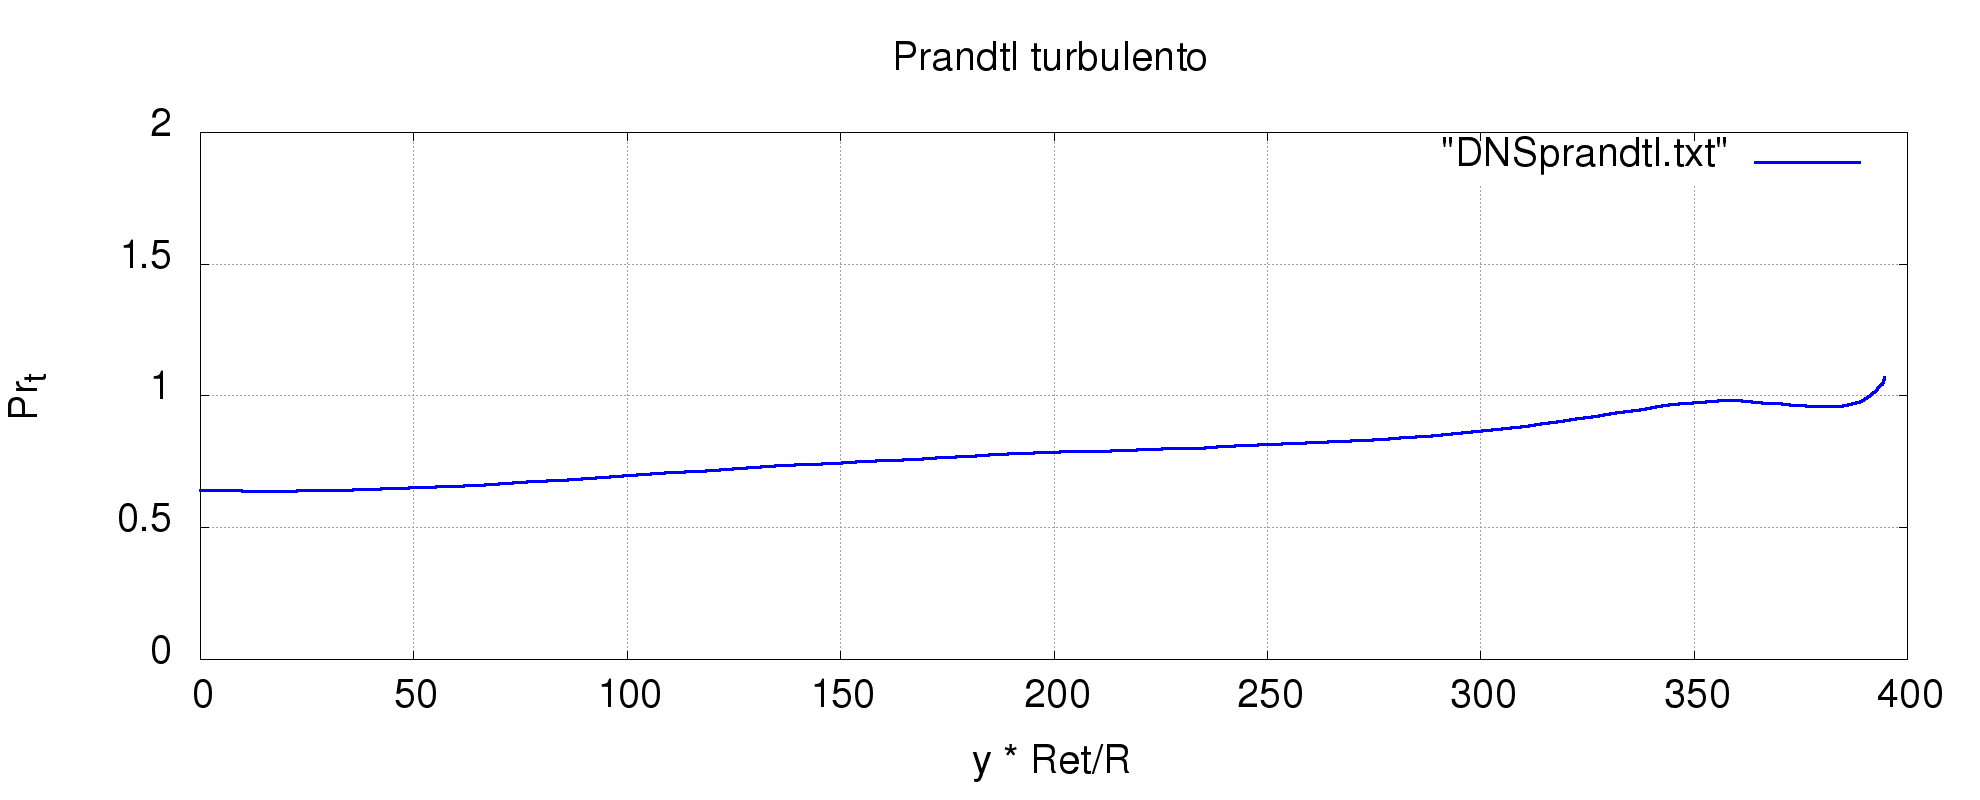
\includegraphics[angle=0, scale=0.25]{perfisPrandtlturb_Ret_Pt}
	\caption{Vector from the DNS with the turbulent Prandtl number according to the coordinate $ y $ in the channel.}
\end{figure*}

Thus, the effort to propose a parameterization adjusted for the turbulent Prandtl number started.
In this sense was tried to adjust a value for which the error was minimal when comparing the simulation with DNS.

\newpage

\subsection{The meta-modeling}
Was wrote an algorithm that searched for a minimal error for the function, considering the turbulent Prandtl number as an editable variable and the smaller error as the pattern of interest.
It obtained a turbulent Prandtl number adjusted of $ 0.905 $ for the turbulent Reynolds number of $ 1020$.
\begin{figure}[!h]
	\centering
	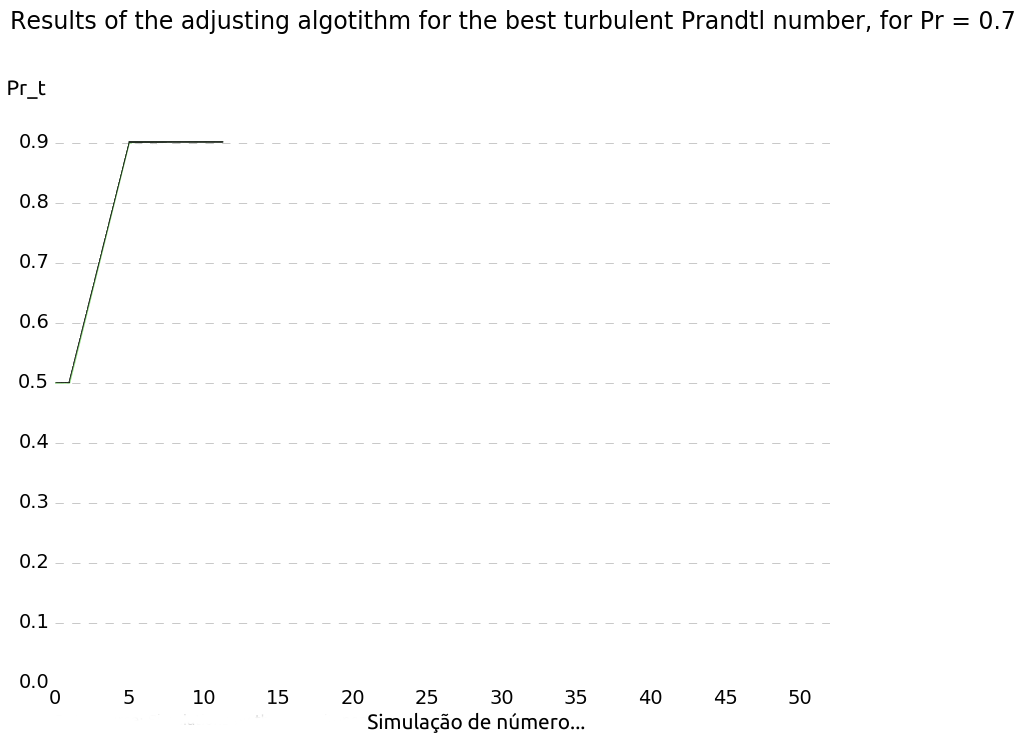
\includegraphics[angle=0, scale=0.25]{oloco}
	\caption{Adjustment algorithm converged on $Pr_t = 0.905$.}
\end{figure}

The value was applied to the entire domain, with the results as follows:
\begin{figure*}[!h]
	\centering
	\begin{subfigure}[t]{0.5\textwidth}
		\centering
		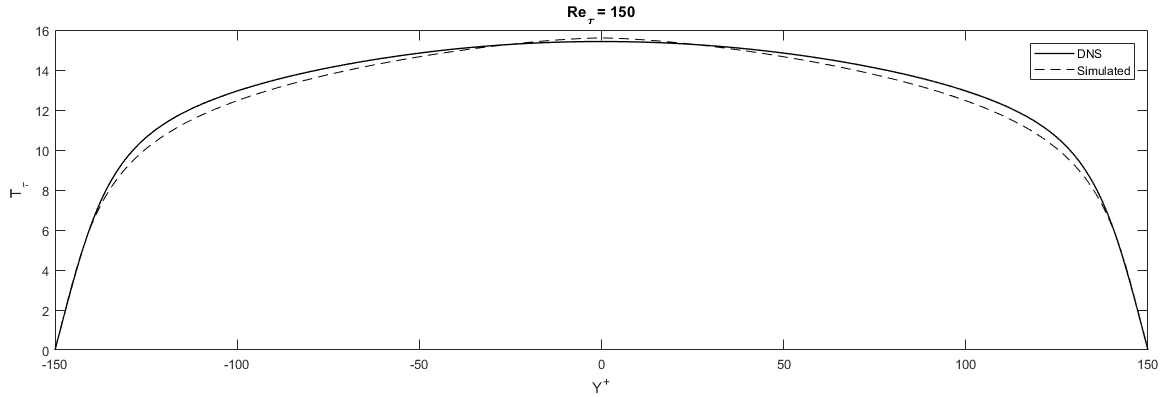
\includegraphics[angle=0, scale=0.24]{150segundo}
		\caption{Results for $Re_\tau = 150$. L2 = 0.341}
	\end{subfigure}
	\begin{subfigure}[t]{0.45\textwidth}
		\centering
		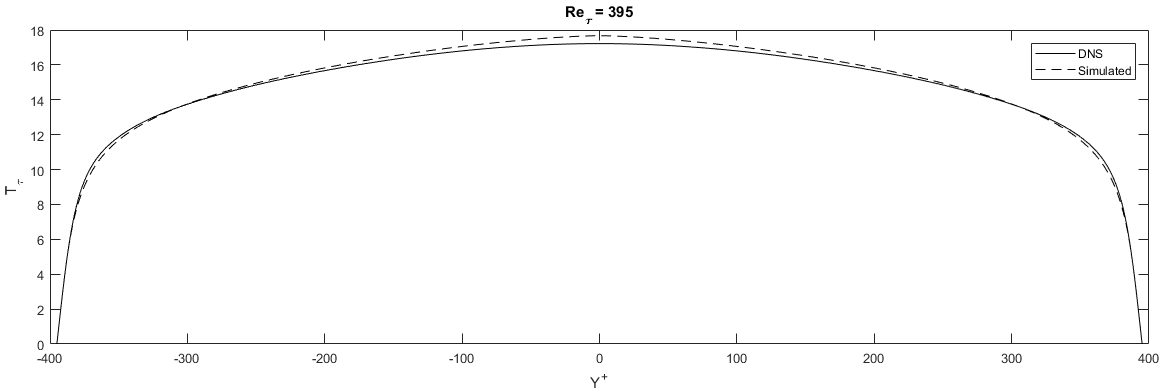
\includegraphics[angle=0, scale=0.24]{395segundo}
		\caption{Results for $Re_\tau = 395$. L2 = 0.23}
	\end{subfigure}
	\begin{subfigure}[t]{0.5\textwidth}
		\centering
		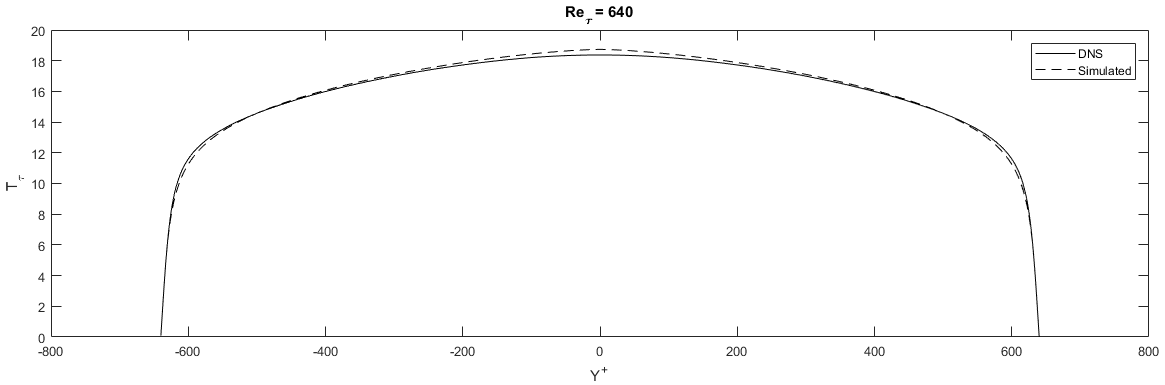
\includegraphics[angle=0, scale=0.24]{640segundo}
		\caption{Results for $Re_\tau = 640$. L2 = 0.192}
	\end{subfigure}
	\begin{subfigure}[t]{0.45\textwidth}
		\centering
		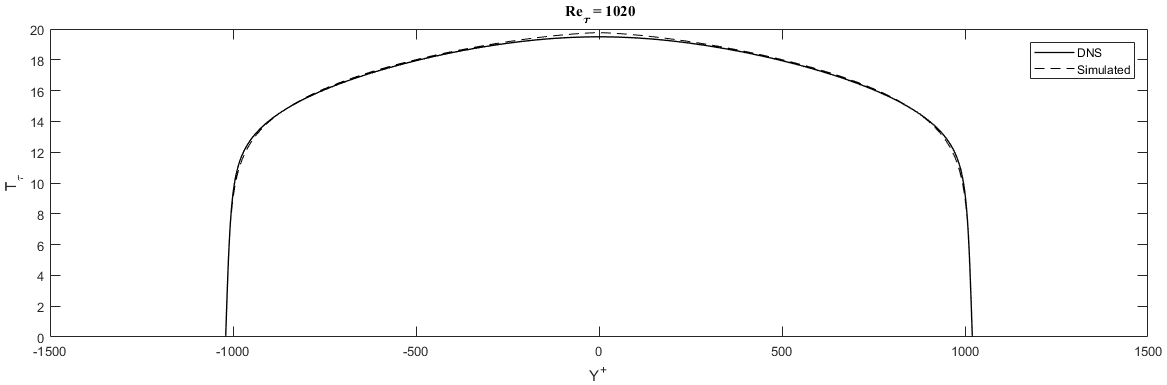
\includegraphics[angle=0, scale=0.24]{1020segundo}
		\caption{Results for $Re_\tau = 1020$. L2 = 0.151}
	\end{subfigure}	
	\caption{Results for $Pr_t = 0.905$ and $A = 26$}
\end{figure*}

Although the results were much better, the model had to be further developed, because the turbulent Prandtl number varies with the Reynolds number, so a model that contemplate this fact had to be created. 
In order to obtain a curve that contemplated the Reynolds numbers throughout the domain, the same optimizing algorithm was used to determine an ideal turbulent Prandtl number for each turbulent Reynolds number available in DNS.

As a way of making sure that a global minimum has been reached, the algorithm was run from a point above and a point below the inferred.	\\

\begin{figure}[!h]
	\centering
	\begin{subfigure}[t]{0.49\textwidth}
		\centering
		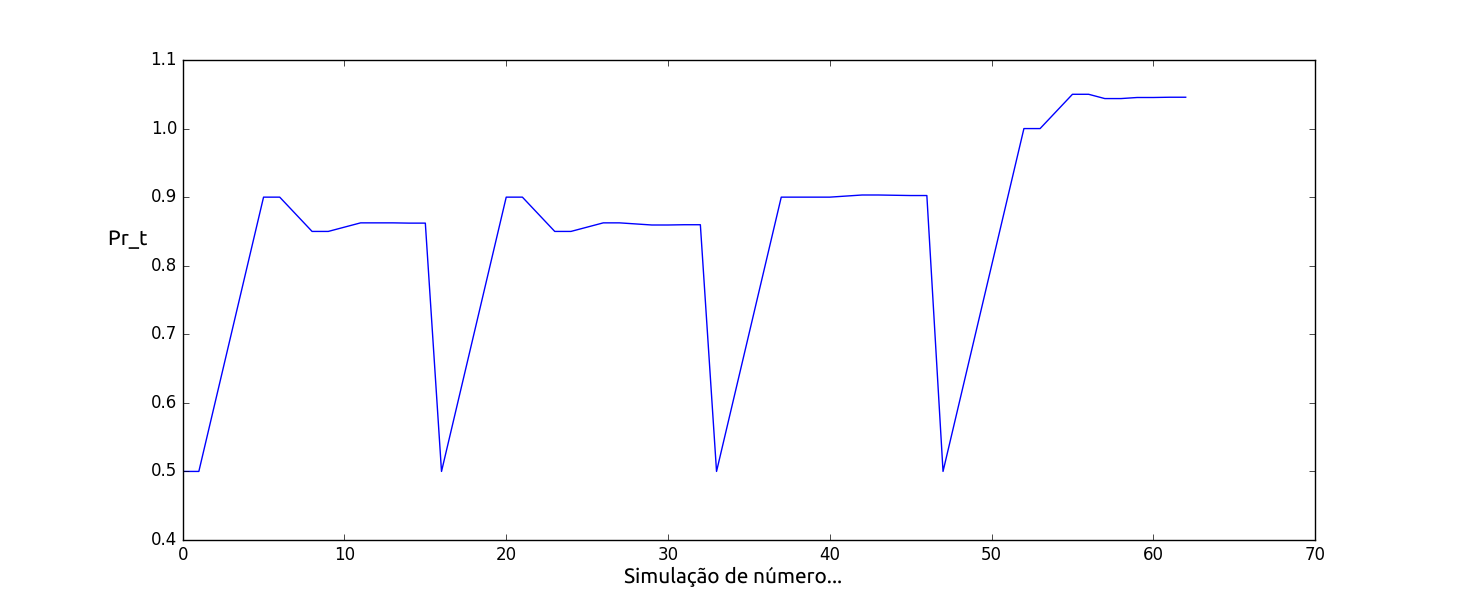
\includegraphics[angle=0, scale=0.19]{convergnciacima}
		\caption{Algorithm for optimal values. With initial value lower than the estimated.}
	\end{subfigure}
	\begin{subfigure}[t]{0.49\textwidth}
		\centering
		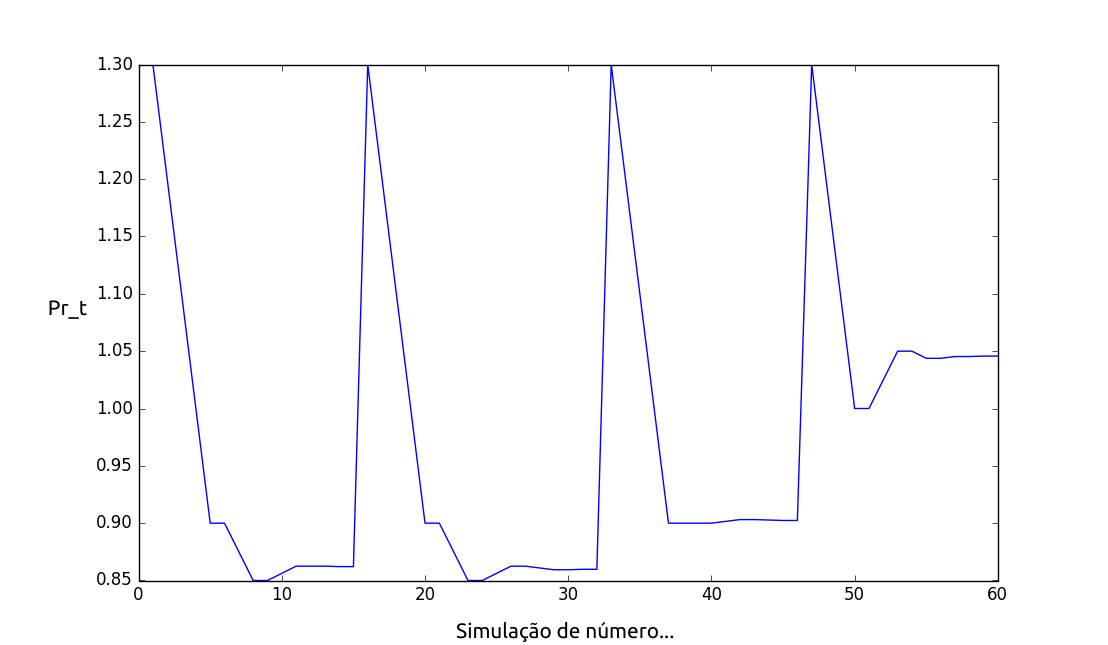
\includegraphics[angle=0, scale=0.19]{convergnciabaixo}
		\caption{Algorithm for optimal values. With initial value greater than the estimated.}
	\end{subfigure}
\caption{Optimization algorithm.}
\end{figure}

By performing a polynomial curve fit, the following relation was obtained:
\begin{equation}
\begin{split}
Pr_t = 1,3 * 10^{-11} Re_\tau^3 - 7,1 * 10^{-8} Re_\tau^2 + 0,0001 Re_\tau + 0,87 
\end{split}
\end{equation}
Thus, a model adjusted for the turbulent Prandtl number as a function of the turbulent Reynolds number was developed.
	\begin{figure}[!h]
	\centering
	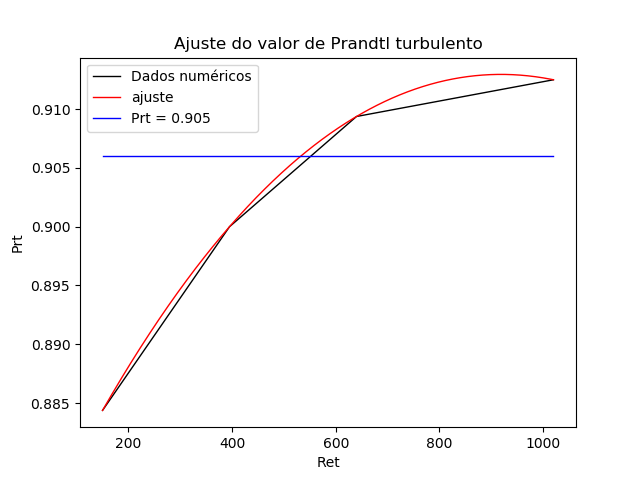
\includegraphics[angle=0, scale=0.295]{ajustePrandtl}
	\caption{Adjust of a model for the $ Pr_t $ variable.}
\end{figure}  


It was studied the velocity profile too, and a adjusted model was created for the Cebeci constant. The same algorithm utilized to find the ideal turbulent Prandtl numbers was used to find an ideal cebecis's constant for each turbulent Reynolds number. 

\begin{figure}[!h]
	\centering
	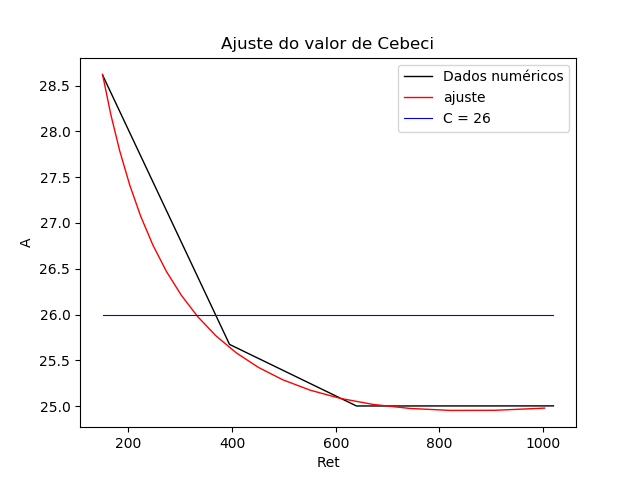
\includegraphics[angle=0, scale=0.295]{ajustecebeci}
	\caption{Adjust of a model for a variable Cebeci's number.}
\end{figure}
 From the resulting points of the optimization algorithm, a model adjusted for the Cebeci value was developed too. As follows:
\begin{equation}
A = \frac{Re_\tau ^{0.0451 * \ln(Re_\tau)} *e ^ {5.2753} }{Re_\tau ^{0.6094}}
\end{equation}
It was studied the influence of the number of molecular Prandtl and it was observed that it was also a variable with influences in the error of the method, thus began a study with the objective of adding the influence of the value of Prandtl number to the parameterization of the turbulent Prandtl number. For this the following model was proposed:
\begin{equation}
\begin{split}
Pr_t = \left( 1,3 * 10^{-11} Re_\tau^3 - 7,1 * 10^{-8} Re_\tau^2 + 0,0001 Re_\tau + 0,87 \right) \left(  \frac{Pr}{0,71}\right) ^{-0.008}
\end{split}
\end{equation}


\section{Results}
With all these methods, a big number of simulations in concerning all the DNS data was made.
Results can be seen ahead.\\
\begin{figure}[!h]
	\centering
	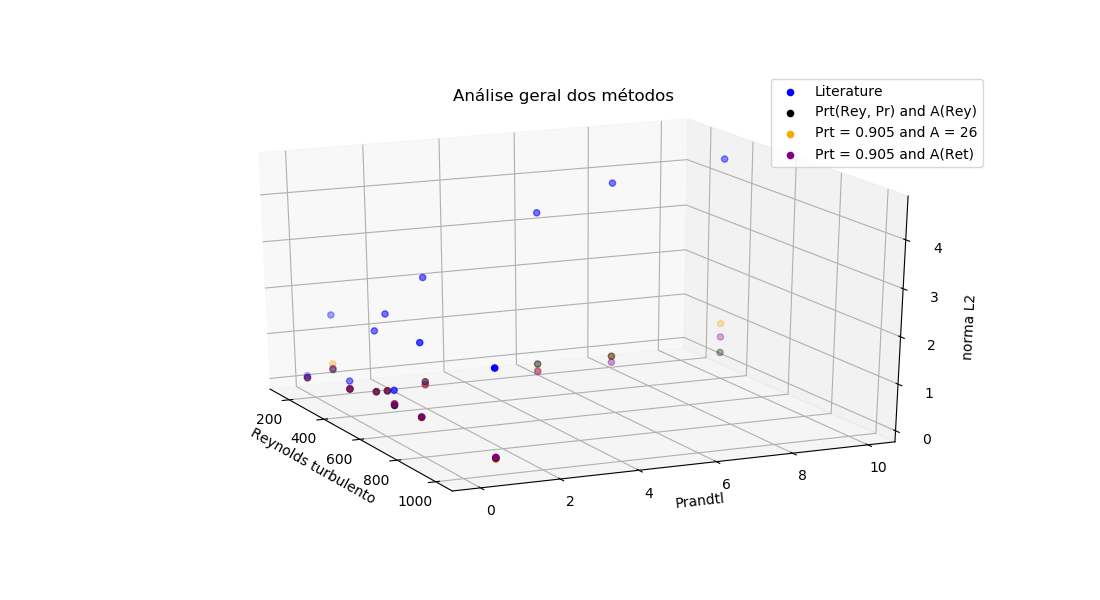
\includegraphics[angle=0, scale=0.42]{finais}
	\caption{Geral results per method.}
\end{figure}
\\
Here are some cuts from the previous chart, explaining the errors obtained for a fixed Ret of 395, and a fixed Pr of 0.71.
\begin{figure}[!h]
	\centering
\begin{subfigure}[t]{0.49\textwidth}
	\centering
	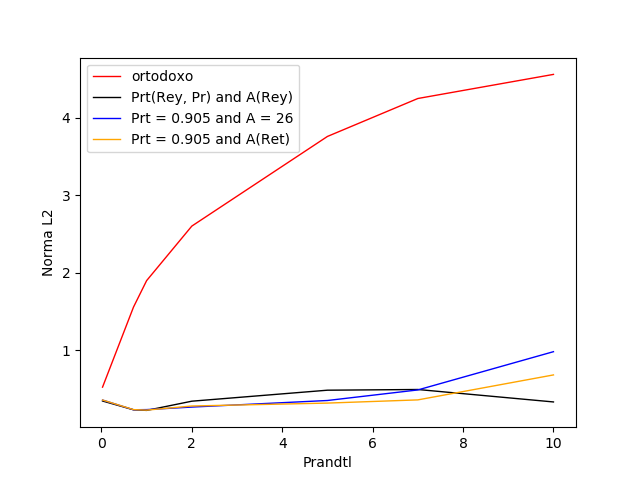
\includegraphics[angle=0, scale=0.35]{finaispr}
	\caption{Results for $Re_\tau = 395$}
\end{subfigure}
\begin{subfigure}[t]{0.49\textwidth}
	\centering
	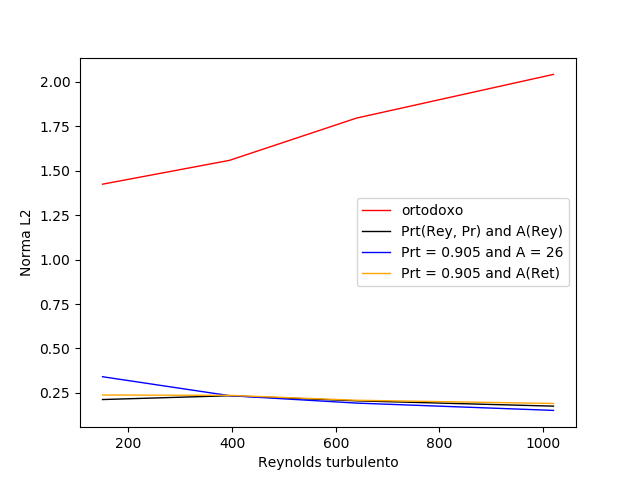
\includegraphics[angle=0, scale=0.35]{finaisRey}
	\caption{Results for $Pr = 0.71$}
\end{subfigure}
\caption{From the 3D plot above.}
\end{figure}

\section{Conclusion}

...

\section{Acknowledgments}

It's opportune to thanks all the institutions involved with the viabilization of this research project. The laboratory of fluids mechanics (Mflab) of the mechanical engineering 
college (FEMEC) of the Federal university of Uberlandia (UFU). PETROBRAS, Cnpq and FAPEMIG that contributed financially to the project.  

\begin{thebibliography}{99} % Bibliography - this is intentionally simple in this template
	
	
	\bibitem{hasan}
	{O. Basim and Hasan}
	\newblock  {"Turbulent Prandtl Number and its Use in Prediction of Heat Transfer Coefficient for liquids."}
	\newblock {Nahrain University, College of engineering Journal (NUCEJ) Vol.10, No.1}
	\newblock {2007}.
	
	
	\bibitem{Poiseuille}
	{J. L. M. Poiseuille},
	\newblock{"Recherches experimentales sur Ie mouvement des liquides dans les tubes de tres-petits diametres"},
	\newblock{Memoires presentes par divers savants a l'Academie Royale des Sciences de l'Institut de France},
	\newblock{IX: 433-544},
	\newblock{1846}.
	
	
	\bibitem{Prandtl}
	\newblock{L. Prandtl},
	\newblock{Uber die ausgebildete Turbulenz},
	\newblock{ZAMM},
	\newblock{1925}.
	
	
	\bibitem{Cebeci}
	{T. Cebeci and P. Bradshaw},
	\newblock{"Physical and computational aspects of convective heat transfer"},
	\newblock{Springer},
	\newblock{New York},
	\newblock{1984}.
	
	
	\bibitem{John}
	\newblock{John C. Sommerer, Edward Ott, et Tamas Tel},
	\newblock{"Modeling Two-Dimensional Fluid Flows with Chaos Theory"},
	\newblock{Johns Hopkins APL Technical Digest, volume 18, number 2},
	\newblock{193-202},
	\newblock{1997}.
	
	
	\bibitem{aristeu}
	\newblock{A. S. {Neto}},
	\newblock{"Turbul\^encia nos fluidos, textbook of the post graduate mechanical engineering course of federal university of Uberl\^andia"},
	\newblock{Uberl\^andia, Brazil},
	\newblock{2018}.
	
	
	\bibitem{Cengel}
	Cengel, Y. A. and Cimbala, J. M.,
	\newblock{Fluid mechanics Fundamentals and Applications},
	\newblock{First edition},
	\newblock{McGraw-Hill series in mechanical engineering},
	\newblock{2006}.
	
	\bibitem{Abe}
	H. Kawamura, H. Abe et Yuichi Matsuo,
	\newblock{DNS of turbulent heat transfer in channel flow with respect to Reynolds and Prandtl number effects},
	\newblock{Elsevier},
	\newblock{Tokio, Japan},
	\newblock{1999}.
	
	
	\bibitem{Kawamura}
	Kawamura, H. , Abe, H. and shingai, k. ,
	\newblock {"DNS of turbulence and heat transport in a channel flow with different Reynolds and Prandtl numbers and boundary conditions."},
	\newblock { Turbulence, Heat and Mass Transfer 3, (Proc. of the 3rd International Symposium on Turbulence, Heat and Mass Transfer)},
	\newblock {2000}.
	
	
	\bibitem{Incropera}
	Incropera, Freank, P., Dewitt, David, P.,  
	\newblock {\em fundamentals of Heat and Mass Transfer}, 3rd edition,
	\newblock p. 310-316, 2007, LTC,
	\newblock (INCROPERA and DEWITT).
	
	\bibitem{DNS1020}
	H Kawamura,
    \newblock{Direct Numerical Simulation Data Base for Turbulent Channel Flow with Heat Transfer.},
	\newblock{<http://www.rs.tus.ac.jp/~t2lab/db/index.html>, Laboratory of Thermo-fluid dynamics, Department of Mechanical Engineering, Faculty of Science and Technology, Tokyo University of Science, Noda-shi, Chiba-ken, Japan},
	\newblock{2007}.	
	
	
	\bibitem{DNS150}
	N Kasagi and K Horiuti and Y Miyake and T Miyauchi and Y Nagano ,
	\newblock{Establishment of the Direct Numerical Simulation Data Bases of Turbulent Transport Phenomena},
	\newblock{<http://thtlab.jp/DNS/dns\_database.html>,  Co-operative Research No. 02302043, Bunkyo-ku, Tokyo 113  },
	\newblock{1992}.	
	
	
\end{thebibliography}





\end{document}
